\documentclass[11pt]{article}
\usepackage[margin=0.75in]{geometry}
\usepackage{amsmath}
\usepackage{enumitem}
\usepackage{color,soul}
\usepackage{multicol}
\usepackage{tikz}

\newcommand{\ds}{\displaystyle}

\begin{document}
\newcounter{enumCount}
\pagestyle{empty}
\subsection*{Math 141 - Homework 3 \hfill Name: \underline{\hspace*{2in}}}

\begin{enumerate}
\item The trapezoid shown below has 3 short sides that are all 10 cm long and one long base.  Find a formula for the length of the base as a function of the angle $\theta$. 
\begin{flushright}
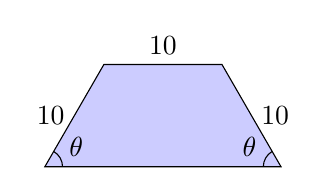
\begin{tikzpicture}[scale=0.15]
\draw (10,8.66) node[above] {10};
\draw (2.5,4.33) node[left] {10};
\draw (17.5,4.33) node[right] {10};
\filldraw[fill=blue!20] (0,0) -- (5,8.66) -- (15,8.66) -- (20,0) -- cycle;
\draw (0,0) node[xshift=0.4cm, yshift=0.25cm] {$\theta$};
\draw (20,0) node[xshift=-0.4cm, yshift=0.25cm] {$\theta$};
\draw (0:1.5) arc(0:60:1.5);
\draw (18.5,0) arc(180:120:1.5);
\end{tikzpicture}
\end{flushright}

\item A telescope on the ground is located 800 meters away from a platform where a rocket launches straight upwards.  The angle of elevation of the telescope as it tracks the rocket is $\theta$.  Find a formula for the distance from the telescope to the rocket as a function of $\theta$. 
\begin{flushright}
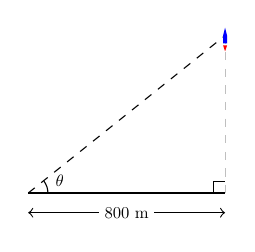
\begin{tikzpicture}[scale=0.5]
\draw (0,0) -- (5,0);
\draw[dashed] (0,0) -- (5,4);
\draw[dashed,gray!50] (5,4) -- (5,0);
\fill[blue] (4.95,3.8) -- (4.95,4) -- (5,4.2) -- (5.05,4) -- (5.05,3.8) -- cycle;
\fill[red] (4.95,3.75) -- (5.05,3.75) -- (5,3.6) -- cycle; 
\draw (4.7,0) -- (4.7,0.3) -- (5,0.3);
\draw[<->] (0,-0.5) -- (5,-0.5);
\draw (0.5,0) arc(0:36.87:0.5);
\draw (0.8,0.3) node[scale=0.6] {$\theta$};
\draw (2.5,-0.5) node[fill=white,scale=0.6] {800 m};
\end{tikzpicture}
\end{flushright}
\setcounter{enumCount}{\theenumi}
\end{enumerate}

\noindent
\textit{For the following exercises, simplify each expression by writing it in terms of sines and cosines, then simplify. The final answer does not have to be in terms of sine and cosine only.}
\begin{multicols}{2}
\begin{enumerate}
\setcounter{enumi}{\theenumCount}
\item $\sec x \sin x \cot x$
\item $\dfrac{\tan^2 \theta}{\sec^2 \theta}$
\setcounter{enumCount}{\theenumi}
\end{enumerate}
\end{multicols}
\vfill

\noindent
\textit{Use the identity $\cos^2 \theta + \sin^2 \theta = 1$ to simplify the following.}
\begin{multicols}{2}
\begin{enumerate}
\setcounter{enumi}{\theenumCount}
\item $\dfrac{1-\sin^2 \alpha}{1- \cos^2 \alpha}$
\item $\dfrac{\cos t}{\sin t} + \dfrac{\sin t}{1+\cos t}$
\setcounter{enumCount}{\theenumi}
\end{enumerate}
\end{multicols}
\vfill

\begin{enumerate}
\setcounter{enumi}{\theenumCount}
\item Consider a stone tossed into the air from ground level with an initial velocity of 40 feet per second. Its height in feet at time t seconds is $h(t)=40t-16t^2$. Consider the average velocity of the stone over the given time intervals. Hint: Use Desmos for this one.
\begin{multicols}{4}
\begin{enumerate}
\item $[1,1.4]$
\item $[1,1.03]$
\item $[1,1.002]$
\item $[1,1.0001]$
\end{enumerate}
\end{multicols}
\vfill

\newpage
\item Use the results from the previous exercise to estimate the instantaneous velocity of the stone at time $t = 1$ second.
\vfill


\noindent 
\item Use the graph below to find the following limits. 
\begin{center}
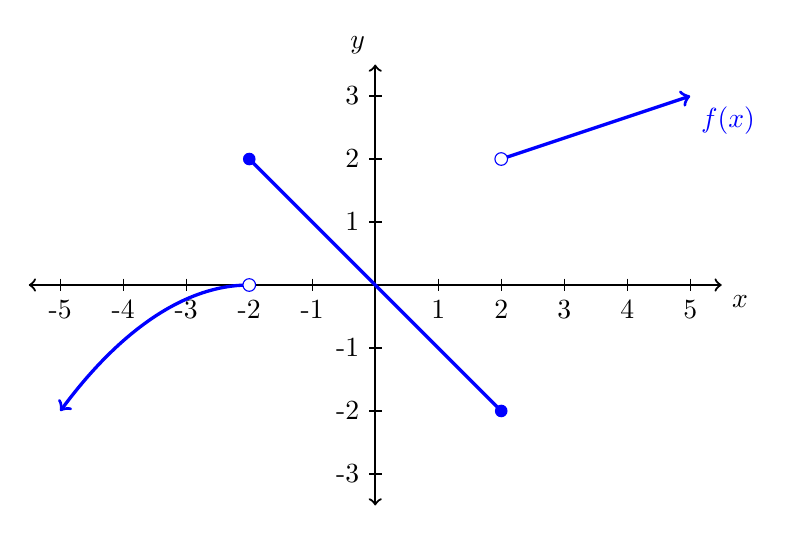
\begin{tikzpicture}[xscale=0.8,yscale=0.8]
\draw[thick,<->] (-5.5,0) -- (5.5,0) node[below right] {$x$};
\draw[thick,<->] (0,-3.5) -- (0,3.5) node[above left] {$y$};
\foreach \x in {1,2,3,4,5} {
  \draw (\x,0.1) -- (\x,-0.1) node[below] {\x};
}
\foreach \x in {-1,-2,-3,-4,-5} {
  \draw (\x,0.1) -- (\x,-0.1) node[below] {\x};
}
\foreach \y in {3,2,1,-1,-2,-3} {
  \draw (0.1,\y) -- (-0.1,\y) node[left] {\y};
}
\draw[very thick, blue, <-] (-5,-2) parabola bend (-2,0) (-2,0);
\draw[very thick, blue] (-2,2) -- (2,-2);
\draw[very thick, blue, ->] (2,2) -- (5,3) node[below right] {$f(x)$};
\filldraw[fill=white,draw=blue] (-2,0) circle (0.1);
\filldraw[fill=white,draw=blue] (2,2) circle (0.1);
\fill[blue] (-2,2) circle (0.1);
\fill[blue] (2,-2) circle (0.1);
\end{tikzpicture}
\end{center}

\begin{multicols}{3}
\begin{enumerate}
\item $\ds \lim_{x \rightarrow -2^-} f(x)$
\item $\ds \lim_{x \rightarrow -2^+} f(x)$
\item $\ds \lim_{x \rightarrow -2} f(x)$
\end{enumerate}
\end{multicols}
\vfill

\begin{multicols}{3}
\begin{enumerate}
\setcounter{enumii}{3}
\item $\ds \lim_{x \rightarrow 2^-} f(x)$
\item $\ds \lim_{x \rightarrow 2^+} f(x)$
\item $\ds \lim_{x \rightarrow 2} f(x)$
\end{enumerate}
\end{multicols}
\vfill

\item The function $f(x) = (1+x)^{1/x}$ is undefined when $x=0$, but the limit $\lim_{x \rightarrow 0} f(x)$ exists.  Graph this function on Desmos, then use the graph to estimate value of the limit (accurate to 3 decimal places).
\vfill
\setcounter{enumCount}{\theenumi}
\end{enumerate}

\end{document}
